\chapter{Impostazione del problema di ricerca}
\label{FormulazioneProblema}
\thispagestyle{empty}

%\begin{quotation}
%{\footnotesize
%\noindent{\emph{``Terence: Rotta a nord con circospezione \\
%Bud: Ehi, gli ordini li do io qui!\\
%Terence: Ok, comante\\
%Bud: Rotta a nord\\
%Terence: Soltanto?\\
%Bud: Con circospezione!''}
%}
%\begin{flushright}
%Chi Trova un Amico Trova un Tesoro
%\end{flushright}
%}
%\end{quotation}
\vspace{0.5cm}
In questo capitolo descriviamo il problema, affrontato dall'algoritmo di tampering detection, in maniera formale e rigorosa. Il primo paragrafo illustra il modello delle osservazioni e gli eventi che siamo interessati a identificare, mentre il secondo paragrafo formalizza il concetto di tampering detection. Nel seguito useremo il termine \textit{vista} per indicare l'ambiente ripreso dalla camera, determinato univocamente dalla posizione della stessa\footnote{Altre volte useremo il termine \textit{inquadratura}.}.
\noindent 
\section{Modello delle osservazioni}
Il nostro campo di osservazione si concentra su quegli eventi che si interpongono tra la scena ripresa da una camera e il sensore che acquisisce le immagini. Non vogliamo, cio\`e, identificare degli eventi particolari che avvengono nella scena, come un oggetto lasciato incustodito \cite{Targhe}, bens\`i vogliamo identificare quegli eventi tali per cui il sensore non \`e pi\`u nelle condizioni di riprendere, in maniera ottimale, la scena, quali ad esempio sfocature o spostamenti della camera.
Nel seguito cerchiamo di dare una definizione formale di questi eventi.
\subsection{Sfocatura}
Il fenomeno della sfocatura avviene quando un elemento trasparente o semitrasparente si interpone tra la lente della camera e la scena ripresa, oppure quando viene cambiata la messa a fuoco, causando una perdita nei dettagli della scena ripresa.

\begin{figure}
	\centering
	\begin{subfigure}[Pioggia sull'obiettivo]
		{\label{fig:pioggia} 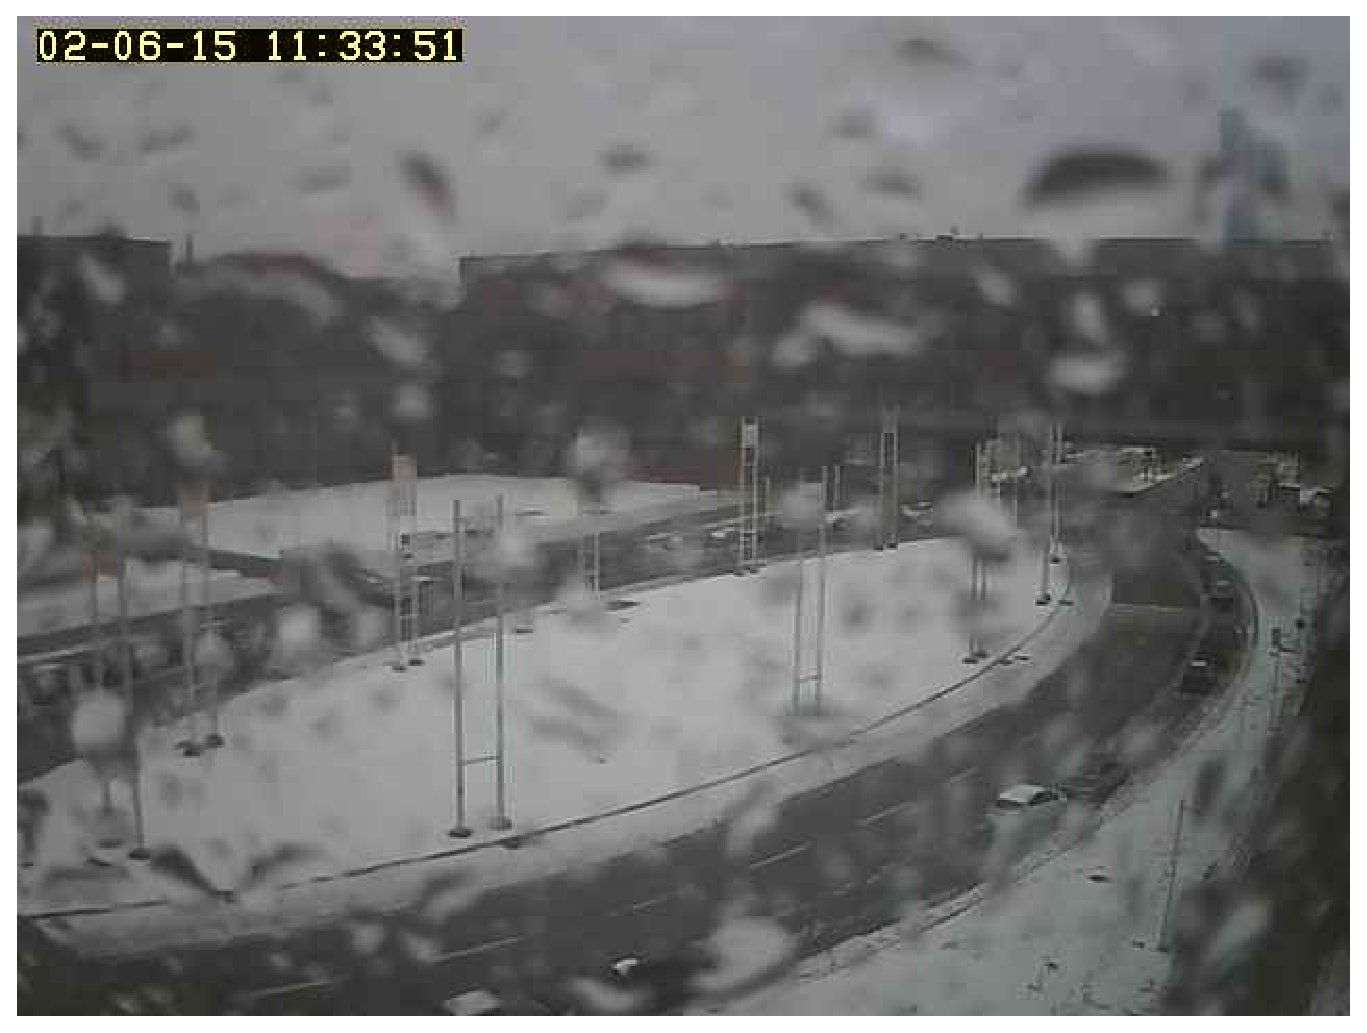
\includegraphics[width=6cm]{./pictures/pioggia}}
	\end{subfigure}
	\begin{subfigure}[Deodorante spray]
		{\label{fig:bassiniDEFOCUS} \includegraphics[width=6cm]{./pictures/bassiniDEFOCUS}}
	\end{subfigure}
	\caption{Esempi di sfocature}
	\label{fig:esempiSfocature}
\end{figure}

\noindent Nella figura \ref{fig:esempiSfocature} sono mostrati degli esempi in cui sono presenti delle sfocature. 
Queste possono essere di origine diversa: 
\begin{itemize}
	\item dovute a \textit{cause naturali}, come ad esempio dell'acqua piovana che si deposita sulla lente (figura \ref{fig:pioggia}), o la condensa dovuta all'umidit\`a e alle basse temperature, oppure un raggio di sole incidente sull'obiettivo della camera;
	\item per \textit{intervento dell'uomo}, che a sua volta pu\`o avvenire in maniera intenzionale (e in questo caso si pu\`o parlare di \textit{manomissione}) oppure non intenzionale. Ad esempio, si pu\`o direttamente intervenire sulla messa a fuoco, nel caso sia possibile cambiarla manualmente; oppure (come nel caso della figura \ref{fig:bassiniDEFOCUS}) \`e possibile applicare una sostanza semitrasparente sulla lente della camera, come il gas di un deodorante spray.
\end{itemize}
Riprendendo \cite{alippi2010detecting}, questo fenomeno pu\`o essere modellato come un operatore di \textit{degradazione} $D$ applicato a un'immagine $y$, considerata priva di errori, i.e.,
\begin{equation}
z=\mathcal{D}[y].
\end{equation}
In particolare, all'interno dell'operatore $\mathcal{D}$ si pu\`o considerare il contributo dovuto a un operatore di \textit{sfocatura} $B$ (dall'inglese \textit{blur}) e un termine aleatorio $\eta$ corrispondente al rumore, i.e.,
\begin{equation}
\label{blur_single}
z(x)=\mathcal{D}[y](x) = \mathcal{B}[y](x) + \eta(x), \qquad x \in \mathcal{X}
\end{equation}
dove abbiamo indicato con $x$ le coordinate dei \textit{pixel} dell'immagine e $\mathcal{X}$ \`e l'insieme dei pixel che formano l'immagine. 
Considerando il caso continuo, possiamo assumere la sfocatura $\mathcal{B}$ come un operatore \textit{lineare},
\begin{equation}
\mathcal{B}[y](x) = \int_{\mathcal{X}}y(s)h(x,s)ds,
\end{equation}
dove $h(x,s)$ rappresenta la \textit{risposta all'impulso} (\textit{point spread function} (PSF)) della sfocatura sul pixel $x$, il cui risultato consiste nel rendere le differenze di intensit\`a, tra pixel adiacenti, pi\`u morbide (\textit{smooth}).
Nel caso in cui la sfocatura sia applicata sulla totalit\`a dell'immagine (come nel caso della figura \ref{fig:bassiniDEFOCUS}), allora \`e possibile modellare l'operatore di blur come una \textit{convoluzione}\footnote{Il blur convoluzionale \`e quello che abbiamo utilizzato per generare, in maniera sintetica, sequenze con immagini sfocate.}:
\begin{equation}
\label{blur_convolution}
\mathcal{B}[y](x) = \int_{\mathcal{X}}y(s)h(s-x)ds,
\end{equation}
dove $h(.)$ \`e un filtro gaussiano o uniforme.\\
Nel caso pi\`u generale possiamo considerare che la camera acquisisca un sequenza di $N$ osservazioni $\{z_i\}, i = 1, \dots ,N$, quindi la formula \ref{blur_single} si pu\`o riscrivere come
\begin{equation}
\label{blur_multi}
z_i(x)=\mathcal{D}_i[y_i](x) = \mathcal{B}_i[y_i](x) + \eta(x), \qquad x \in \mathcal{X}.
\end{equation}

La sequenza delle immagini $\{y_i\}, i = 1,\dots , N$, pu\`o variare in maniera significativa nel suo contenuto, anche nel caso in cui la vista sia la stessa.
\begin{figure}
	\centering
	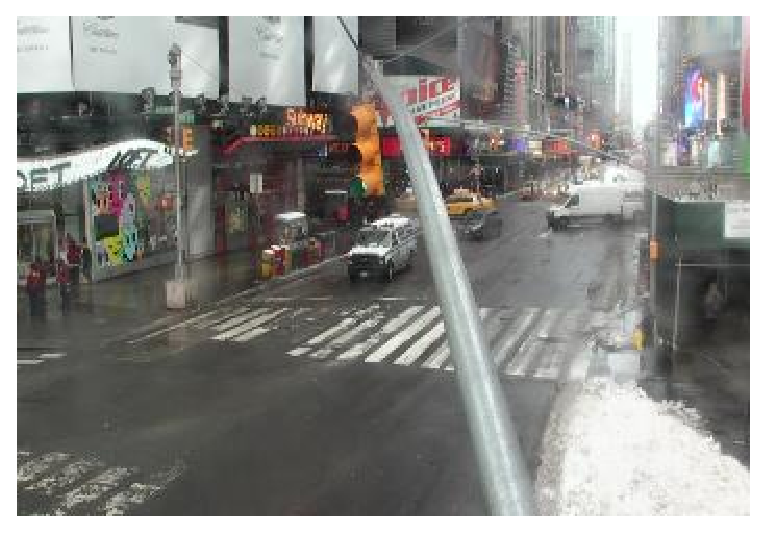
\includegraphics[width=3cm]{./pictures/image0001.eps}
	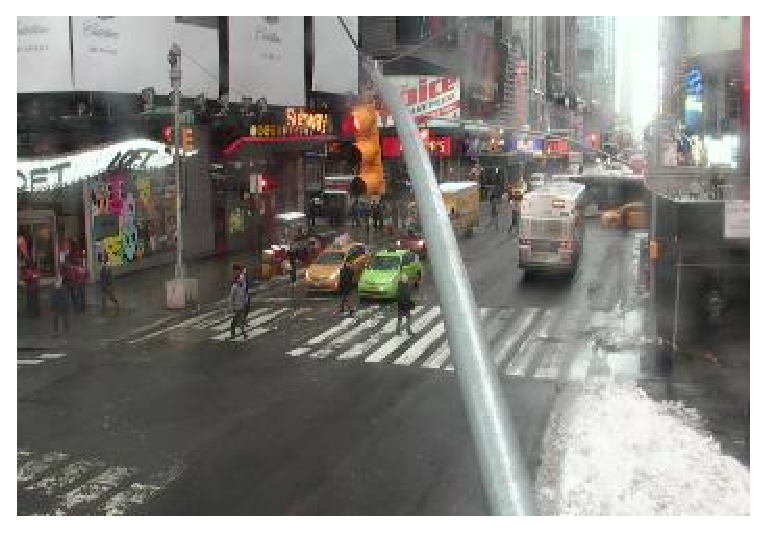
\includegraphics[width=3cm]{./pictures/image0002.eps}
	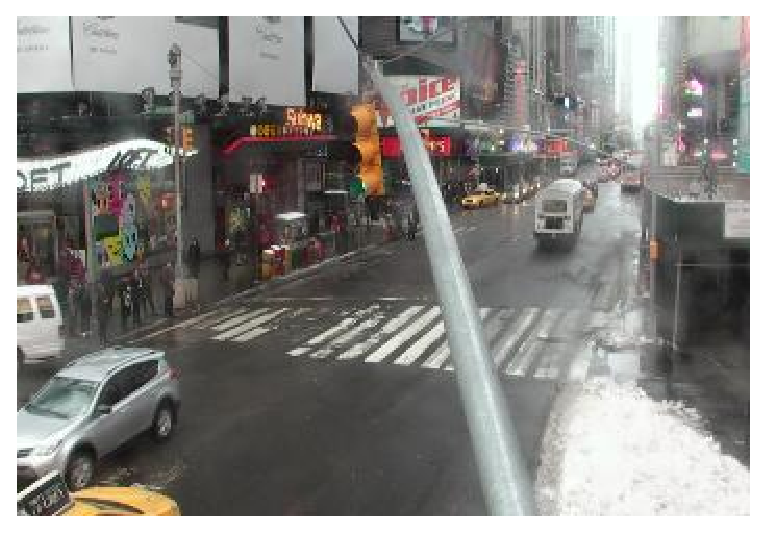
\includegraphics[width=3cm]{./pictures/image0003.eps}
	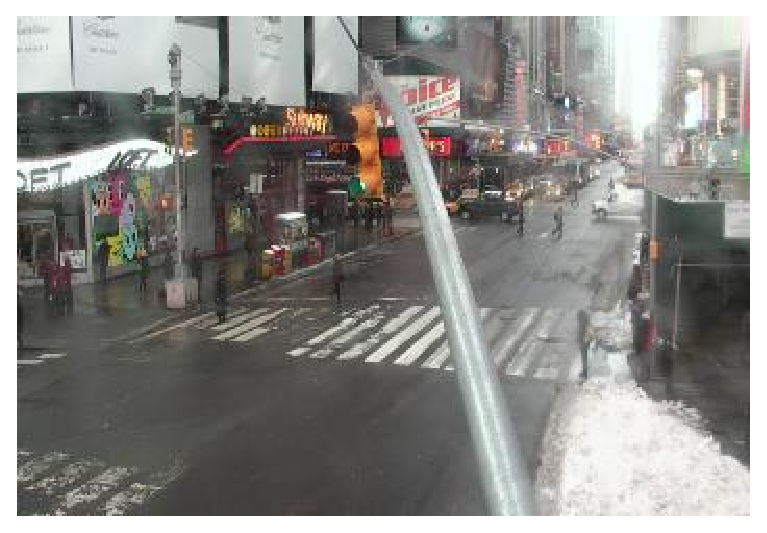
\includegraphics[width=3cm]{./pictures/image0004.eps}
	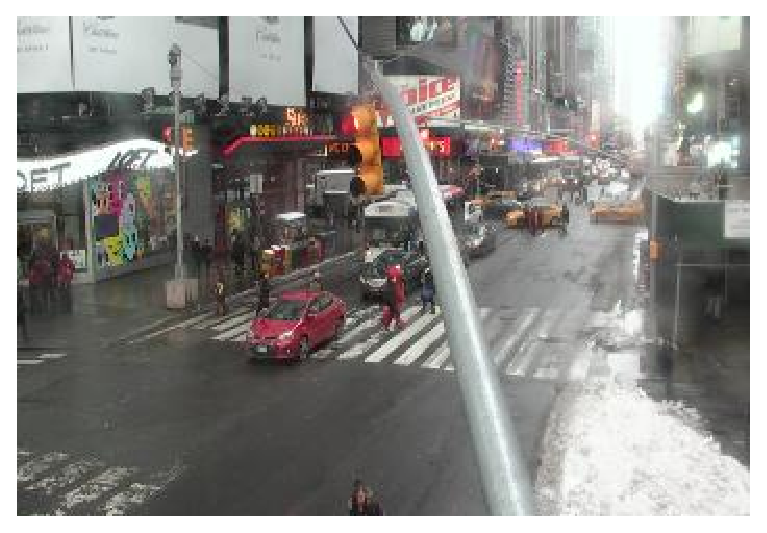
\includegraphics[width=3cm]{./pictures/image0005.eps}
	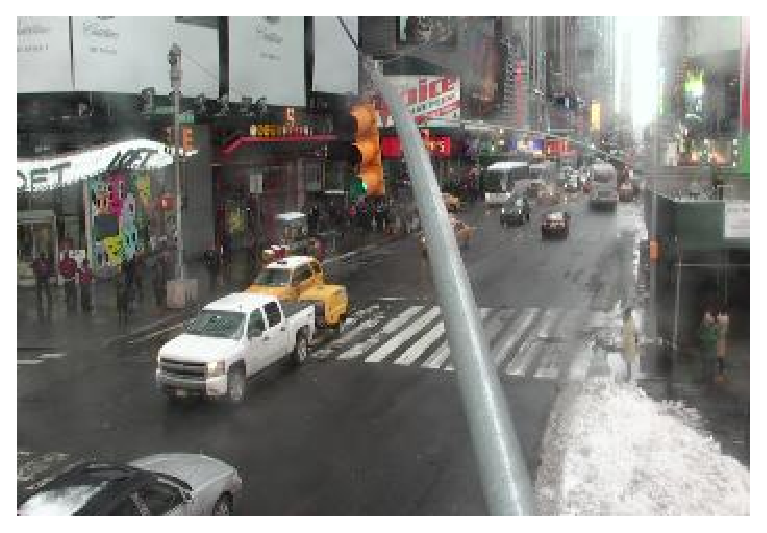
\includegraphics[width=3cm]{./pictures/image0006.eps}
	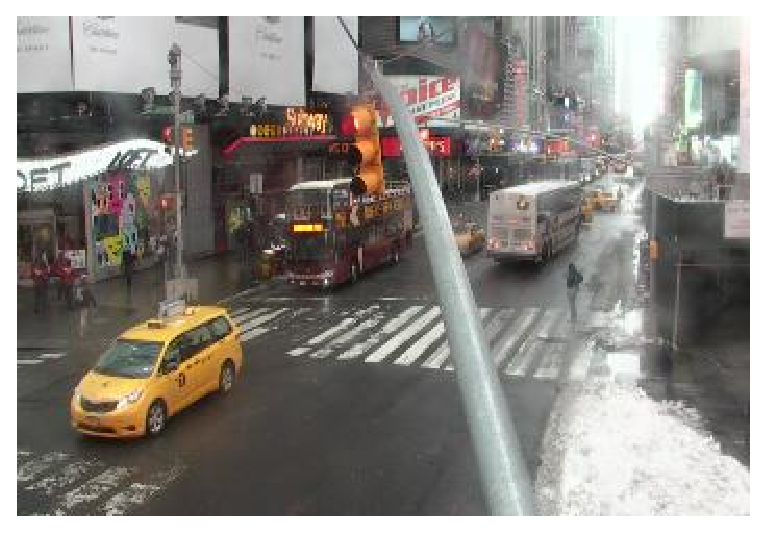
\includegraphics[width=3cm]{./pictures/image0007.eps}
	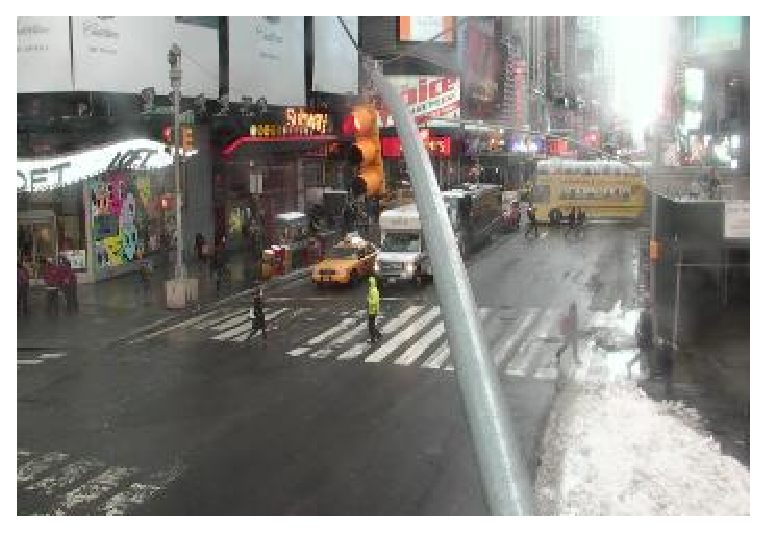
\includegraphics[width=3cm]{./pictures/image0008.eps}
	\caption{Sequenza di otto frame consecutivi acquisiti ogni minuto}
	\label{fig:framDifferences}
\end{figure}
\noindent Un esempio \`e illustrato nella figura \ref{fig:framDifferences}, in cui le immagini riprese dalla camera sono acquisite ogni minuto. 
Nonostante l'inquadratura non cambi tra le acquisizioni, il contenuto delle singole immagini varia parecchio, dato il continuo passaggio di automobili e pedoni.
Questo problema fa s\`i che l'identificazione delle sfocature non possa avvenire facendo un semplice confronto tra frame consecutivi, in quanto avremmo un numero troppo elevato di falsi positivi.
Infatti, nel caso in cui avessimo un riscontro negativo dal confronto tra due frame ($z_i \neq z_{i + 1}$), sarebbe difficile capire se \`e cambiato il contenuto delle immagini ($y_i \neq y_{i + 1}$) o l'operatore di sfocatura ($\mathcal{B}_i \neq \mathcal{B}_{i + 1}$). 
\subsection{Spostamento della camera}
Lo spostamento della camera avviene quando cambia la sua vista.
Le cause possono essere, ancora una volta, di tipo naturale, ad esempio una raffica di vento che sposta la camera, oppure dovute a un intervento malevolo da parte di un uomo.
\begin{figure}
	\centering
	\subfigure[Vista originale]{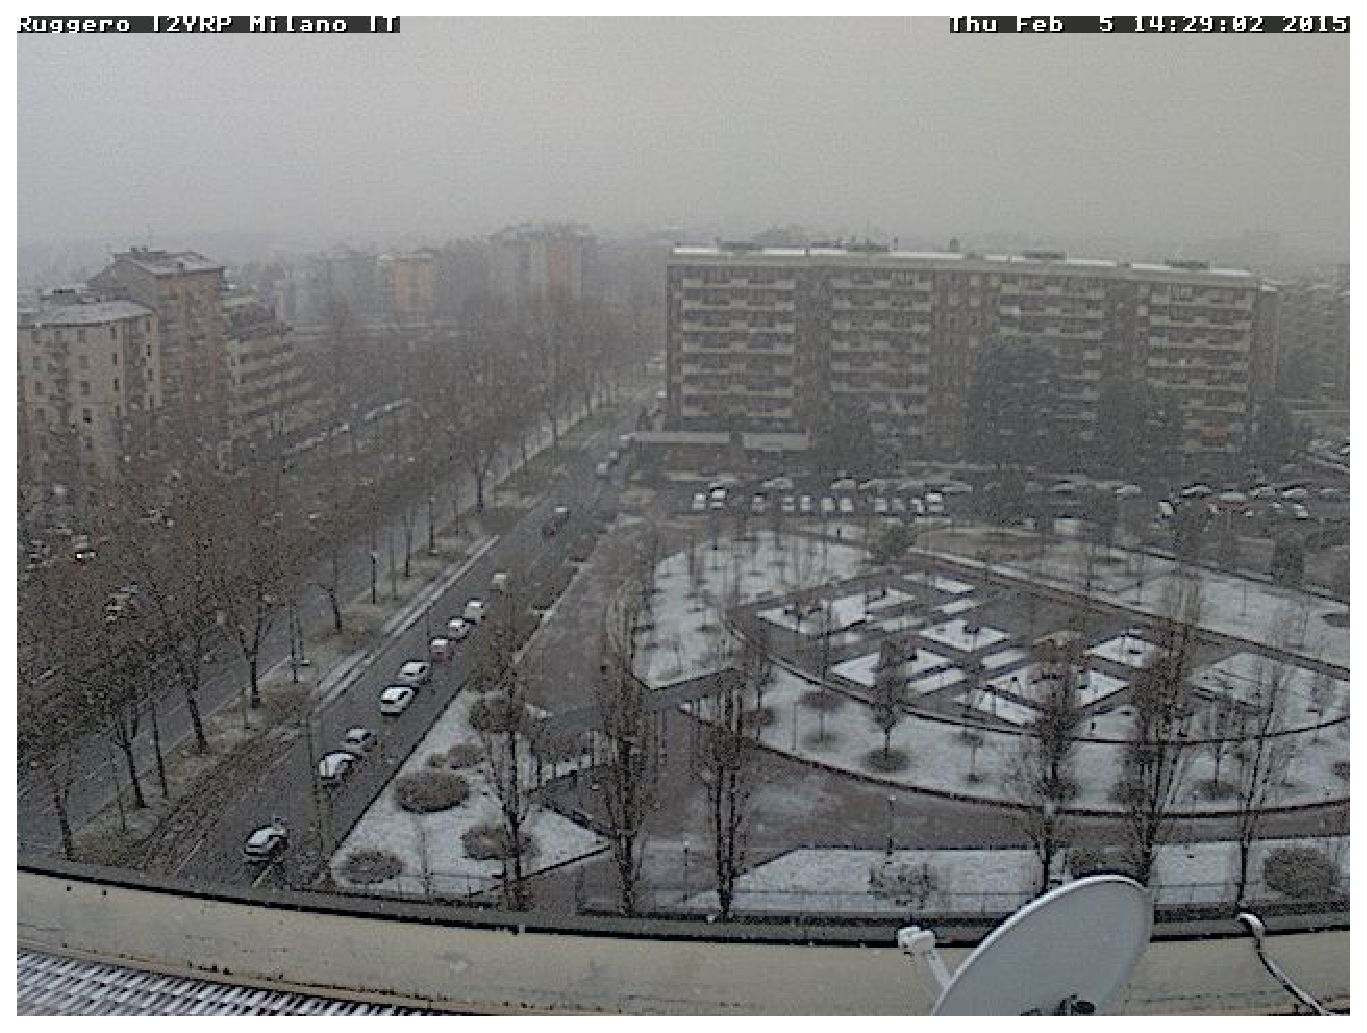
\includegraphics[width=6cm]{./pictures/testiORIGINALE}}
	\subfigure[Vista in seguito allo spostamento della camera]{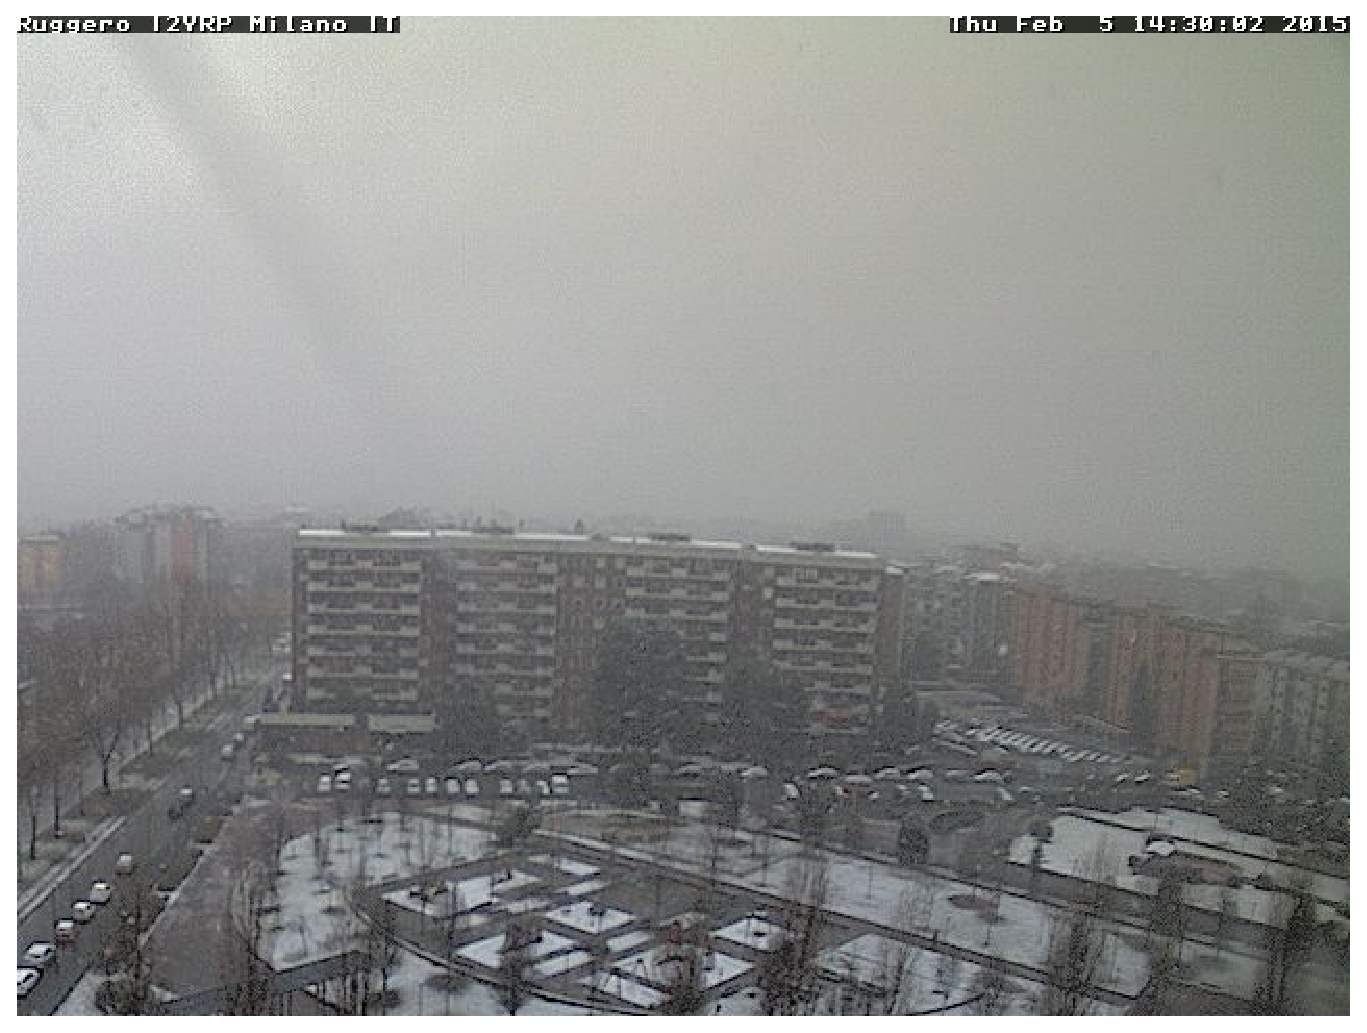
\includegraphics[width=6cm]{./pictures/testiDISPLACEMENT}}
	\caption{Esempio di spostamento della camera}
	\label{fig:testiDISPLACEMENT}
\end{figure}
\noindent Un esempio di spostamento della camera \`e mostrato nella figura \ref{fig:testiDISPLACEMENT}.
Possiamo formalizzare il concetto di spostamento della camera nel modo seguente: consideriamo la sequenza $\{y_i\}$ di immagini generate da una camera in una certa posizione, e la sequenza $\{w_i\}$ di immagini generate dalla stessa camera in una posizione differente.\\
Possiamo, dunque, considerare la sequenza di immagini $\{z_i\}$ in cui avviene uno spostamento della camera all'istante $T^*$ nel seguente modo:
\begin{equation}
\label{eq:displacement}
z_i(x) = \left\{ \begin{array}{rcl}
	y_i(x) + \eta(x) & \mbox{per} & i < T^* \\
	w_i(x) + \eta(x) & \mbox{per} & i \geqslant T^*,
	\end{array}\right.
\end{equation}
dove $\eta(x)$ \`e un rumore stazionario.\\
Anche per lo spostamento della camera vale la considerazione fatta nel caso della sfocatura: il contenuto delle immagini varia con il passare del tempo, quindi identificare lo spostamento confrontando frame consecutivi nel tempo genera un alto numero di falsi positivi.
\subsection{Occlusione e guasti della camera}
Il fenomeno dell'occlusione avviene quando un oggetto opaco si pone a ridosso della camera, impedendo la visione di una parte, se non la totalit\`a, della scena. 
\section{Tampering detection}
